\chapter{Active Directory/LDAP Configuration}

In order to facilitate single signon for users, the details of the directory service must be registered with Obidos.
This can be Active Directory or LDAP.
More than one Configuration can be stored in Obidos.

\section{New AD/LDAP Configuration}

In order to create a new Configuration, select "Create AD/LDAP Settings" from the top level "Settings" menu.

\begin{figure}[H]
\centering
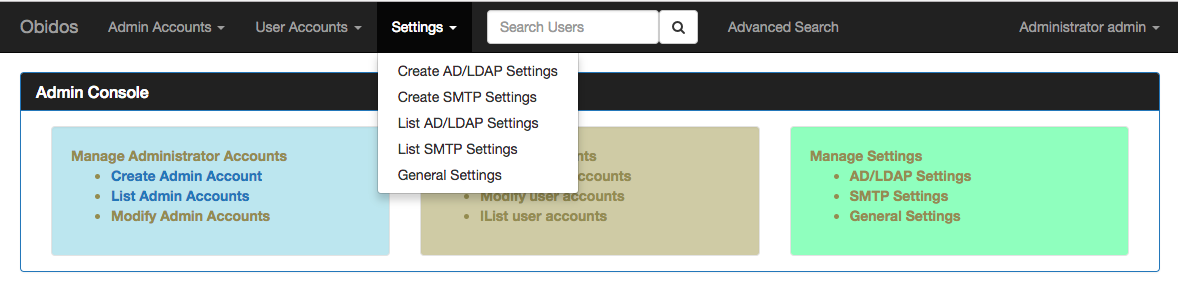
\includegraphics[width=90mm]{admin/Settings-Menu.png}
\caption{Menu for new AD/LDAP Configuration}
\label{fig: Figure}
\end{figure}

The resulting screen to input the fields for a Configuration are as shown in the following figure.

\begin{figure}[H]
\centering
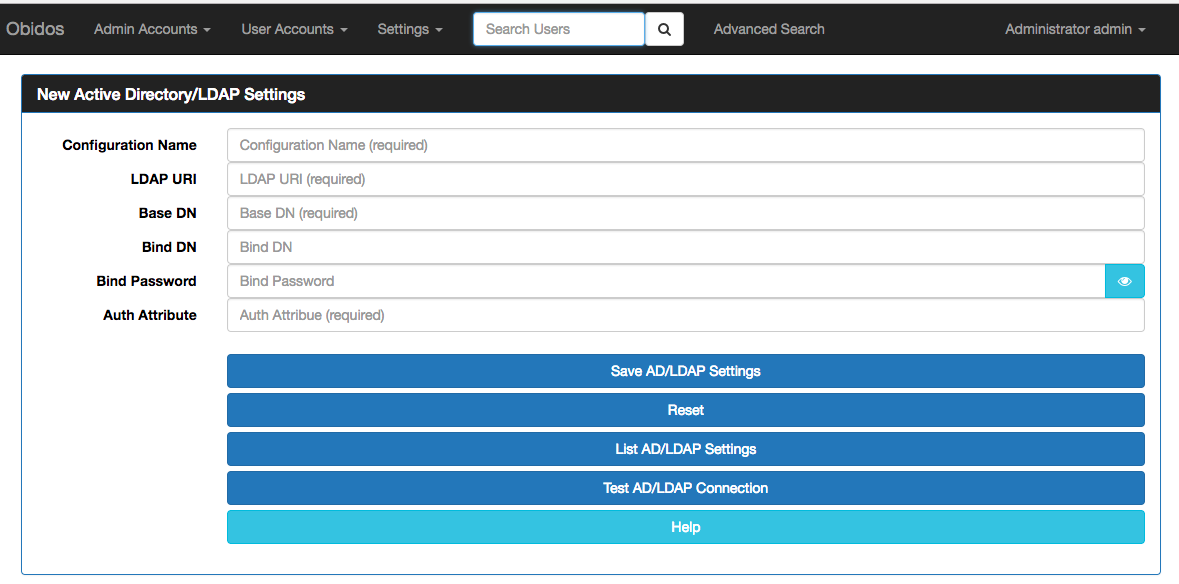
\includegraphics[width=90mm]{admin/Directory-Details.png}
\caption{Fields for Directory Service}
\label{fig: Figure}
\end{figure}

The Configuration Name is the identifier for the Configuration.
This will be used to identify the Directory service for single signon when a user account is created.

The LDAP URI field is usually of the form ldap://\textless hostname \textgreater:\textless port \textgreater. 
\\*An example is ldap://spenego.com:389, where 389 is the port for the LDAP server.

